\section{Benjamin--Bona--Mahony (BBM) Equation}
\label{sec:bbm-experiment}

In this section, we turn to a one-dimensional nonlinear BBM experiment, originally introduced as a regularised long-wave model by Benjamin, Bona, andMahony~\cite{BBM}. It tests the automated space--time localisation for a nonlinear dispersive equation, for which the nonlinear DWR identity is required. Moreover, it tests whether the entity recovery remains complete when the time derivative is paired through a spatial $H^1$ bilinear form rather than the spatial $L^2$ pairing used in the previous heat and advection--diffusion examples.


\subsection{Primal Problem and Solitary Wave}

Let $\Omega=(0,L)$ and impose periodic boundary conditions by identifying $x=0$ with $x=L$. The spatial domain is the one-dimensional torus
\[
  \Omega = \mathbb T_L\coloneqq\mathbb R/(L\mathbb Z).
  \label{eq:bbm-periodic-domain}
\]
The torus notation records that the two endpoints are the same physical point: there is no exterior spatial boundary, and the periodic seam is treated as an interior facet. The unforced BBM equation is
\begin{equation}
  u_t-u_{xxt}+u_x+u u_x=0
  \qquad\text{in }\Omega\times(0,T],
  \label{eq:bbm-strong}
\end{equation}
or, equivalently,
\begin{equation}
  (I-\partial_{xx})u_t
  +\partial_x\left(u+\frac12u^2\right)=0.
  \label{eq:bbm-conservative}
\end{equation}
The spatial bilinear form associated with the time derivative is
\begin{equation}
  m_{\mathrm{BBM}}(w,v)
  \coloneqq(w,v)_\Omega+(\partial_xw,\partial_xv)_\Omega,
  \label{eq:bbm-h1-mass}
\end{equation}
which is an $H^1$-type spatial mass pairing. 

% The weak problem is to find $u(t)\in H^1_{\mathrm{per}}(\Omega)$ such that
% \begin{equation}
%   m_{\mathrm{BBM}}(u_t,v)
%   -\left(u+\frac12u^2,\partial_xv\right)_\Omega=0
%   \qquad
%   \forall v\in H^1_{\mathrm{per}}(\Omega).
%   \label{eq:bbm-weak}
% \end{equation}

For $c\in(0,1)$, BBM admits the solitary-wave solution on the real line
\begin{equation}
  u_{\mathrm{sol}}(x,t)
  =\frac{3c^2}{1-c^2}
   \operatorname{sech}^2\!\left[
    \frac c2\left(x-x_0-\frac{t}{1-c^2}\right)
   \right].
  \label{eq:bbm-solitary-wave}
\end{equation}
We take $L=100$, $c=0.5$, and $x_0=30$. The amplitude is one and the propagation speed is
\[
  s=\frac{1}{1-c^2}=\frac43.
  \label{eq:bbm-wave-speed}
\]
Thus the wave centre moves from $x_0=30$ to $x_0+sT=54$ at $T=18$.
%\pef{Does that matter?}
% Its exponentially small tails therefore make the long periodic computation a close approximation to the solitary wave on the real line.


\subsection{Quantity of Interest}

We take the terminal quantity of interest
\begin{equation}
  J(u)=(\psi,u(T))_\Omega,
  \label{eq:bbm-qoi}
\end{equation}
where
\begin{equation}
    \psi(x)=\exp\!\left[-\left(\frac{x-x_s}{r_s}\right)^2\right],
  \qquad x_s=54,\qquad r_s=1.
  \label{eq:bbm-sensor}
\end{equation}
It measures the wave in a narrow neighbourhood of its predicted terminal position and is therefore sensitive to phase, amplitude, and shape errors near the sensor. High-order quadrature of the solitary wave gives
\begin{equation}
J_{\mathrm{ref}}=J(u_{\mathrm{sol}})=1.7203.
  \label{eq:bbm-reference-goal}
\end{equation}

% Since the solitary-wave solution is known analytically, the reference quantity of interest can be evaluated independently of the finite element discretisation. Specifically, we compute
% \begin{equation}
%   J_{\mathrm{ref}}
%   =
%   \int_0^L
%   \exp\left(
%     -\left(\frac{x-x_s}{r_s}\right)^2
%   \right)
%   u_{\mathrm{sol}}(x,T)\,\mathrm{d}x
%   =
%   1.7202507189,
%   \label{eq:bbm-reference-goal}
% \end{equation}
% using a 512-point Gauss--Legendre quadrature rule.  Doubling the quadrature order changes the result by less than $3\times10^{-14}$. Thus, the quadrature error is negligible relative to the reported goal-functional discretisation errors.


% adjoint sensitivity
% Let $U$ be the state about which the nonlinear equation is linearised and set $\tau=T-t$.  In reverse time, the adjoint weak problem is
% \begin{equation}
%   m_{\mathrm{BBM}}(\partial_\tau z,w)
%   -\bigl((1+U(T-\tau))\partial_xz,w\bigr)_\Omega=0
%   \qquad
%   \forall w\in H^1_{\mathrm{per}}(\Omega),
%   \label{eq:bbm-adjoint}
% \end{equation}
% with terminal condition
% \begin{equation}
%   m_{\mathrm{BBM}}(z(T),w)=(\psi,w)_\Omega.
%   \label{eq:bbm-adjoint-terminal}
% \end{equation}
% Consequently, $z(T)$ is the $H^1$ Riesz representative of the Gaussian sensor, not its pointwise interpolation. It is smoother and wider than $\psi$.  Its backward propagation forms a dispersive sensitivity corridor; the DWR indicator is expected to be large where this corridor overlaps the forward trajectory $x=x_0+st$.


\subsection{Localisation: Mixed Space--Time Ridge}
\label{sec:bbm-mixed-ridge-specialisation}

This subsection identifies the additional support entity. The derivation is used only to interpret the weak functional: the implementation continues to evaluate and project the original weak residual and does not insert a case-specific strong-residual formula.

Let
\begin{equation}
  j_n=u_h(t_{n-1}^{+})-P_nu_h(t_{n-1}^{-})
  \label{eq:bbm-discrete-jump}
\end{equation}
be the dG interface defect, including transfer $P_n$ from the preceding slab when consecutive slabs use different spatial meshes. For the spatial $L^2$ mass pairing used by the heat and standard advection--diffusion problems, the dG jump contributes
\begin{equation}
  \rho_{n,L^2}^{\mathrm{tf}}(v)=-(j_n,v(t_{n-1}^{+}))_\Omega.
  \label{eq:bbm-l2-interface-contrast}
\end{equation}
Thus the jump itself acts only on the value trace over the temporal face.

For BBM the same defect is paired through \eqref{eq:bbm-h1-mass}:
\begin{equation}
  \rho_n^{\mathrm{tf}}(v)
  =-\sum_{K\in\mathcal T_n}
   \left[(j_n,v)_K+(\partial_xj_n,\partial_xv)_K\right].
  \label{eq:bbm-temporal-residual}
\end{equation}
The derivative term acts over the temporal face in the original weak form. Its cellwise distributional interpretation is
\begin{equation}
  \rho_n^{\mathrm{tf}}(v)
  =\sum_{K\in\mathcal T_n}(-j_n+\partial_{xx}j_n,v)_K
   -\sum_{F\in\mathcal F_n^{\mathrm{int}}}
    ([\![\partial_xj_n]\!],v)_F.
  \label{eq:bbm-temporal-ibp}
\end{equation}
The first sum is supported on $K\times\{t_{n-1}\}$, the interior of a temporal face. The second is supported on
\begin{equation}
  F\times\{t_{n-1}\},
  \label{eq:bbm-mixed-entity}
\end{equation}
the intersection of a spatial facet and the temporal interface. This is the mixed space--time ridge. In one spatial dimension a facet $F$ is a point, so the mixed ridge appears as a zero-dimensional space--time corner in the $(x,t)$ diagram.

For the present cG1 discretisation, $j_n$ is piecewise linear. Therefore
\begin{equation*}
  \partial_{xx}j_n=0\quad\text{inside each cell},
  \qquad
  [\![\partial_xj_n]\!]_F\ne0\quad\text{in general}.
  \label{eq:bbm-cg1-ridge}
\end{equation*}
The derivative part of the interface defect can consequently have a substantial mixed-ridge component.

% In the bubble recovery, the temporal-face interior is represented by $B_xC_t$, while the remaining facet--time interaction is represented by $C_xC_t$. The mixed mode is obtained as the non-vanishing remainder after the volume, spatial-trace, and temporal-trace stages.  It is therefore found by the general entity-recursive algorithm rather than manually inserted from \eqref{eq:bbm-temporal-ibp}. The ablation experiment below tests whether this mode is numerically necessary.


\subsection{Results and Interpretation}

The global estimator uses the nonlinear DWR identity~\cref{eq:practical-nonlinear-estimator}. The low-order and enriched spaces are, respectively,
\begin{equation*}
  V_h^{\mathrm{low}}=\mathrm{cG}(1)\otimes\mathrm{dG}(0),
  \qquad
  V_h^+=\mathrm{cG}(2)\otimes\mathrm{dG}(1).
  % \label{eq:bbm-discrete-spaces}
\end{equation*}
We take the D\"orfler marking fraction as $0.35$ and bisect a time slab when at least $10\%$ of its spatial cells are selected. We have initially $50$ spatial cells and $6$ time slabs. The terminal time is set to be $T = 18$.

To verify algebraic completeness as stated in \cref{sec:bbm-mixed-ridge-specialisation}, each adaptive iterate is post-processed on the same primal solution, adjoint solution, and mesh in two ways: with all recovered entities and after deleting only the signed mixed-ridge contribution.
% Define
% \begin{equation}
%   \delta_{\mathrm{loc}}
%   \coloneqq\sum_{n,K}\eta_{K,n}-\eta_{\mathrm{global}}.
%   \label{eq:bbm-localisation-gap}
% \end{equation}
% With the mixed ridge included, $|\delta_{\mathrm{loc}}|$ stays at floating-point roundoff, but without it it does not. For example, deleting only the mixed-ridge term rises to about \(12.7\%\) at iteration~12. 
Including the mixed-ridge contribution yields global--local agreement up to floating-point roundoff, whereas omitting only this contribution produces a relative localisation gap of approximately \(12.7\%\) at iteration~12.

%This test in \cref{tab:bbm-mixed-ridge-ablation} demonstrates that the mixed ridge term is required to reproduce the global DWR estimator for this BBM calculation.
%\begin{table}[h]
%  \centering
%  \begin{tabular}{rrrrr}
%    \toprule
%    Iteration
%    & Space--time cells
%    & \(\left|\delta_{\mathrm{loc}}\right|\)
%    & \(\left|\delta_{\mathrm{loc}}^{\mathrm{no\,mix}}\right|\)
%    & \(\frac{ \left|\delta_{\mathrm{loc}}^{\mathrm{no\,mix}}\right|}{\left|\eta_{\mathrm{global}}\right|}\)\\
%    \midrule
%     0 &  300 & \(4.44\times10^{-16}\) & \(2.85\times10^{-2}\) & \(3.33\%\) \\
%     4 &  350 & \(5.55\times10^{-16}\) & \(3.07\times10^{-2}\) & \(3.56\%\) \\
%     8 &  856 & \(9.99\times10^{-16}\) & \(5.11\times10^{-2}\) & \(5.65\%\) \\
%    12 & 2816 & \(2.11\times10^{-15}\) & \(6.47\times10^{-2}\) & \(8.78\%\) \\
%    \bottomrule
%  \end{tabular}
%  \caption{Mixed-ridge ablation performed on identical discrete primal and adjoint solutions.}
%  \label{tab:bbm-mixed-ridge-ablation}
%\end{table}

% \begin{figure}[h]
%   \centering
%   \includegraphics[width=0.76\linewidth]
%     {figures/bbm_mixed_ridge_ablation.pdf}
%   \caption{Localisation-gap ablation on identical discrete solutions.}
%   \label{fig:bbm-mixed-ridge-ablation}
% \end{figure}

\Cref{fig:bbm-mesh-evolution} displays the adapted meshes in the $(x,t)$ plane. The initial mesh is uniform. At iteration \(6\), local spatial and temporal refinements form a recognisable diagonal corridor from the initial wave position towards the terminal sensor. By iteration $12$, this corridor is substantially denser, while cells far from it remain comparatively coarse. Its alignment with the exact space--time wave whose centre moves from $x=30$ at $t=0$ to $x=54$ at $T=18$.

\begin{figure}[!htbp]
  \centering
  % space--time axis
  \begin{subfigure}[b]{0.05\textwidth}
  \centering
    \begin{tikzpicture}[>=latex, line width=0.6pt, scale=0.8]
      \draw[->] (0,0) -- (0,0.6) node[above=1pt] {$t$};
      \draw[->] (0,0) -- (0.6,0) node[right=1pt] {$x$};
    \end{tikzpicture}
    \vspace{-1.5em}
    \captionsetup{labelformat=empty}
    \caption*{\strut}
  \end{subfigure}
  \hfill
  \begin{subfigure}[b]{0.90\linewidth}
    \centering
    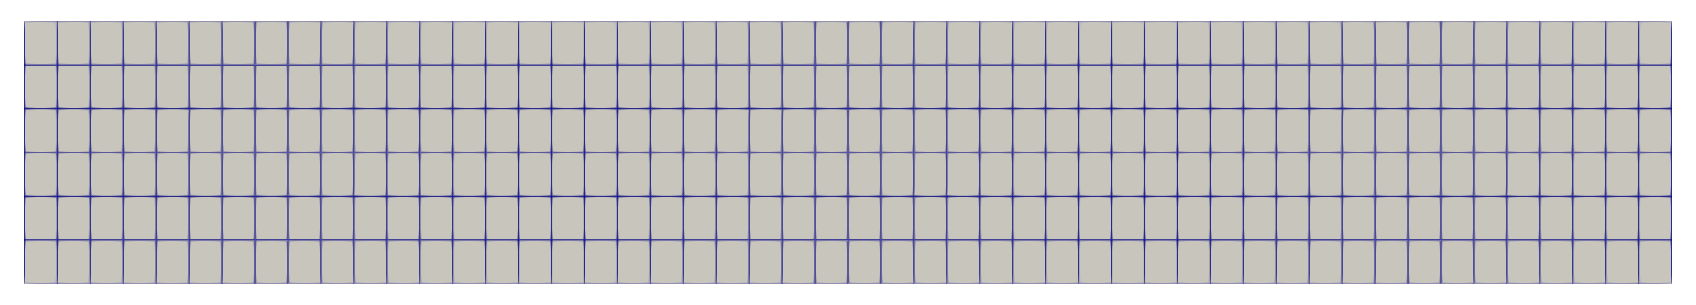
\includegraphics[width=\linewidth, height=0.25\textheight, keepaspectratio]{figures/bbm/bbm_mesh_iter_00.png}
    \caption{Iteration 0: 300 space--time cells.}
  \end{subfigure}
  \vspace{0.5em}
  
  \begin{subfigure}[b]{0.90\linewidth}
    \centering
    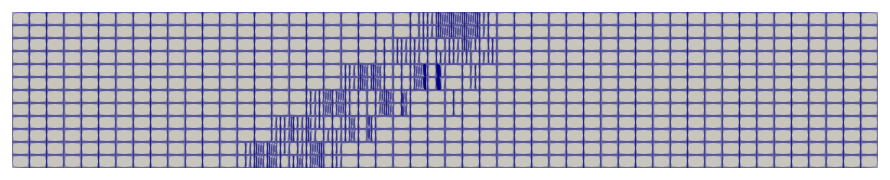
\includegraphics[width=\linewidth, height=0.25\textheight, keepaspectratio]{figures/bbm/bbm_mesh_iter_06.png}
    \caption{Iteration 6: 870 space--time cells.}
  \end{subfigure}
  \vspace{0.5em}

  \begin{subfigure}[b]{0.90\linewidth}
    \centering
    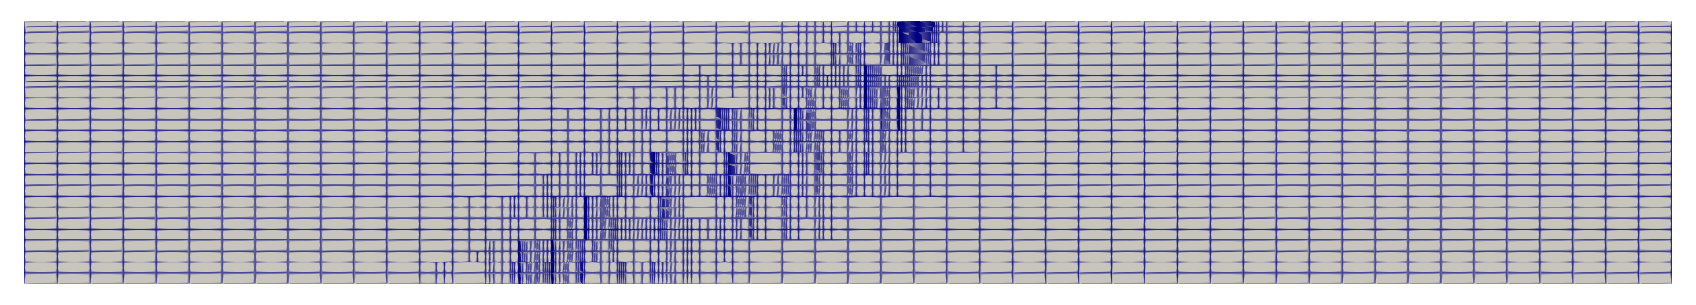
\includegraphics[width=\linewidth, height=0.25\textheight, keepaspectratio]{figures/bbm/bbm_mesh_iter_12.png}
    \caption{Iteration 12: 10{,}431 space--time cells.}
  \end{subfigure}
  \caption{Evolution of the independently refined slabwise space--time mesh.}
  \label{fig:bbm-mesh-evolution}
\end{figure}

Finally, selected iterations up to iteration \(12\) are reported in \cref{tab:bbm-results}. Over this sequence, the goal error decreases from \(1.1720\) to \(4.1940\times10^{-1}\), while the global effectivity index improves from \(0.7306\) to \(0.9806\). 
% Finally, selected iterations are reported in \cref{tab:bbm-results}. The goal error decreases from its initial value to \(9.1811\times10^{-2}\) at iteration \(18\). The global effectivity index improves from \(0.7306\) initially to \(0.9868\) at iteration \(9\), but subsequently decreases to \(0.9000\) on the final mesh. Although this remains a satisfactory effectivity index, the downward trend indicates a moderate underestimation of the goal error at later refinement levels. This may reflect the limited accuracy of the enriched approximations under strongly non-uniform space--time refinement, together with the higher-order terms omitted from the two-term DWR estimator. Nevertheless, the estimator continues to capture both the magnitude and the decay of the goal error.
\begin{table}[!htbp]
\centering
\small
\setlength{\tabcolsep}{4pt}
\begin{tabular}{lllllrr}
\toprule
Iter. & Space--time cells &
$N_t$ & Terminal DoFs & $\lvert J_{\mathrm{ref}}-J(u_h)\rvert$ & $\eta_{\mathrm{global}}$ & $I_{\mathrm{eff}}^{\mathrm{glob}}$ \\
\midrule
 0 &     300 &     6 &    50 & $1.1720$                   & $8.5624\times10^{-1}$ & 0.7306 \\
 3 & 346 & 6 & 58 & $1.1662$ & $8.6313\times10^{-1}$ & 0.7401 \\
 6 &     870 &    12 &    73 & $9.7814\times10^{-1}$     & $9.0395\times10^{-1}$ & 0.9242 \\
 9 &   2,545 &    27 &   111 & $7.4250\times10^{-1}$     & $7.3270\times10^{-1}$ & 0.9868 \\
12 &  10,431 &    81 &   263 & $4.1940\times10^{-1}$     & $4.1126\times10^{-1}$ & 0.9806 \\
% 15 &  42,552 &   206 &   861 & $1.9764\times10^{-1}$     & $1.8692\times10^{-1}$ & 0.9458 \\
% 18 & 189,670 &   601 & 1,956 & $9.1811\times10^{-2}$     & $8.2626\times10^{-2}$ & 0.9000 \\
% 20 & 530,315 & 1,208 & 3,757 & $5.2067\times10^{-2}$     & $4.5028\times10^{-2}$ & 0.8648 \\
\bottomrule
\end{tabular}
\caption{Selected iterations of the periodic BBM adaptive calculation.}
\label{tab:bbm-results}
\end{table}
%\pef{Can we do more adaptive iterations? These computations should be fairly cheap, I think?}
%\yue{More iterations are included in the table. The temporal bisection went crazy so I stopped at 20}

% \begin{figure}[htbp]
%   \centering
%   \includegraphics[width=0.76\linewidth]{figures/bbm_effectivity.pdf}
%   \caption{Effectivity of the symmetric nonlinear DWR estimator.}
%   \label{fig:bbm-effectivity}
% \end{figure}
